\begin{document}
\chapter{Interfaccia Applicazione}\label{app:gui}
\begin{figure}[H]
  \centerline{
    \begin{subfigure}{0.33\textwidth}
      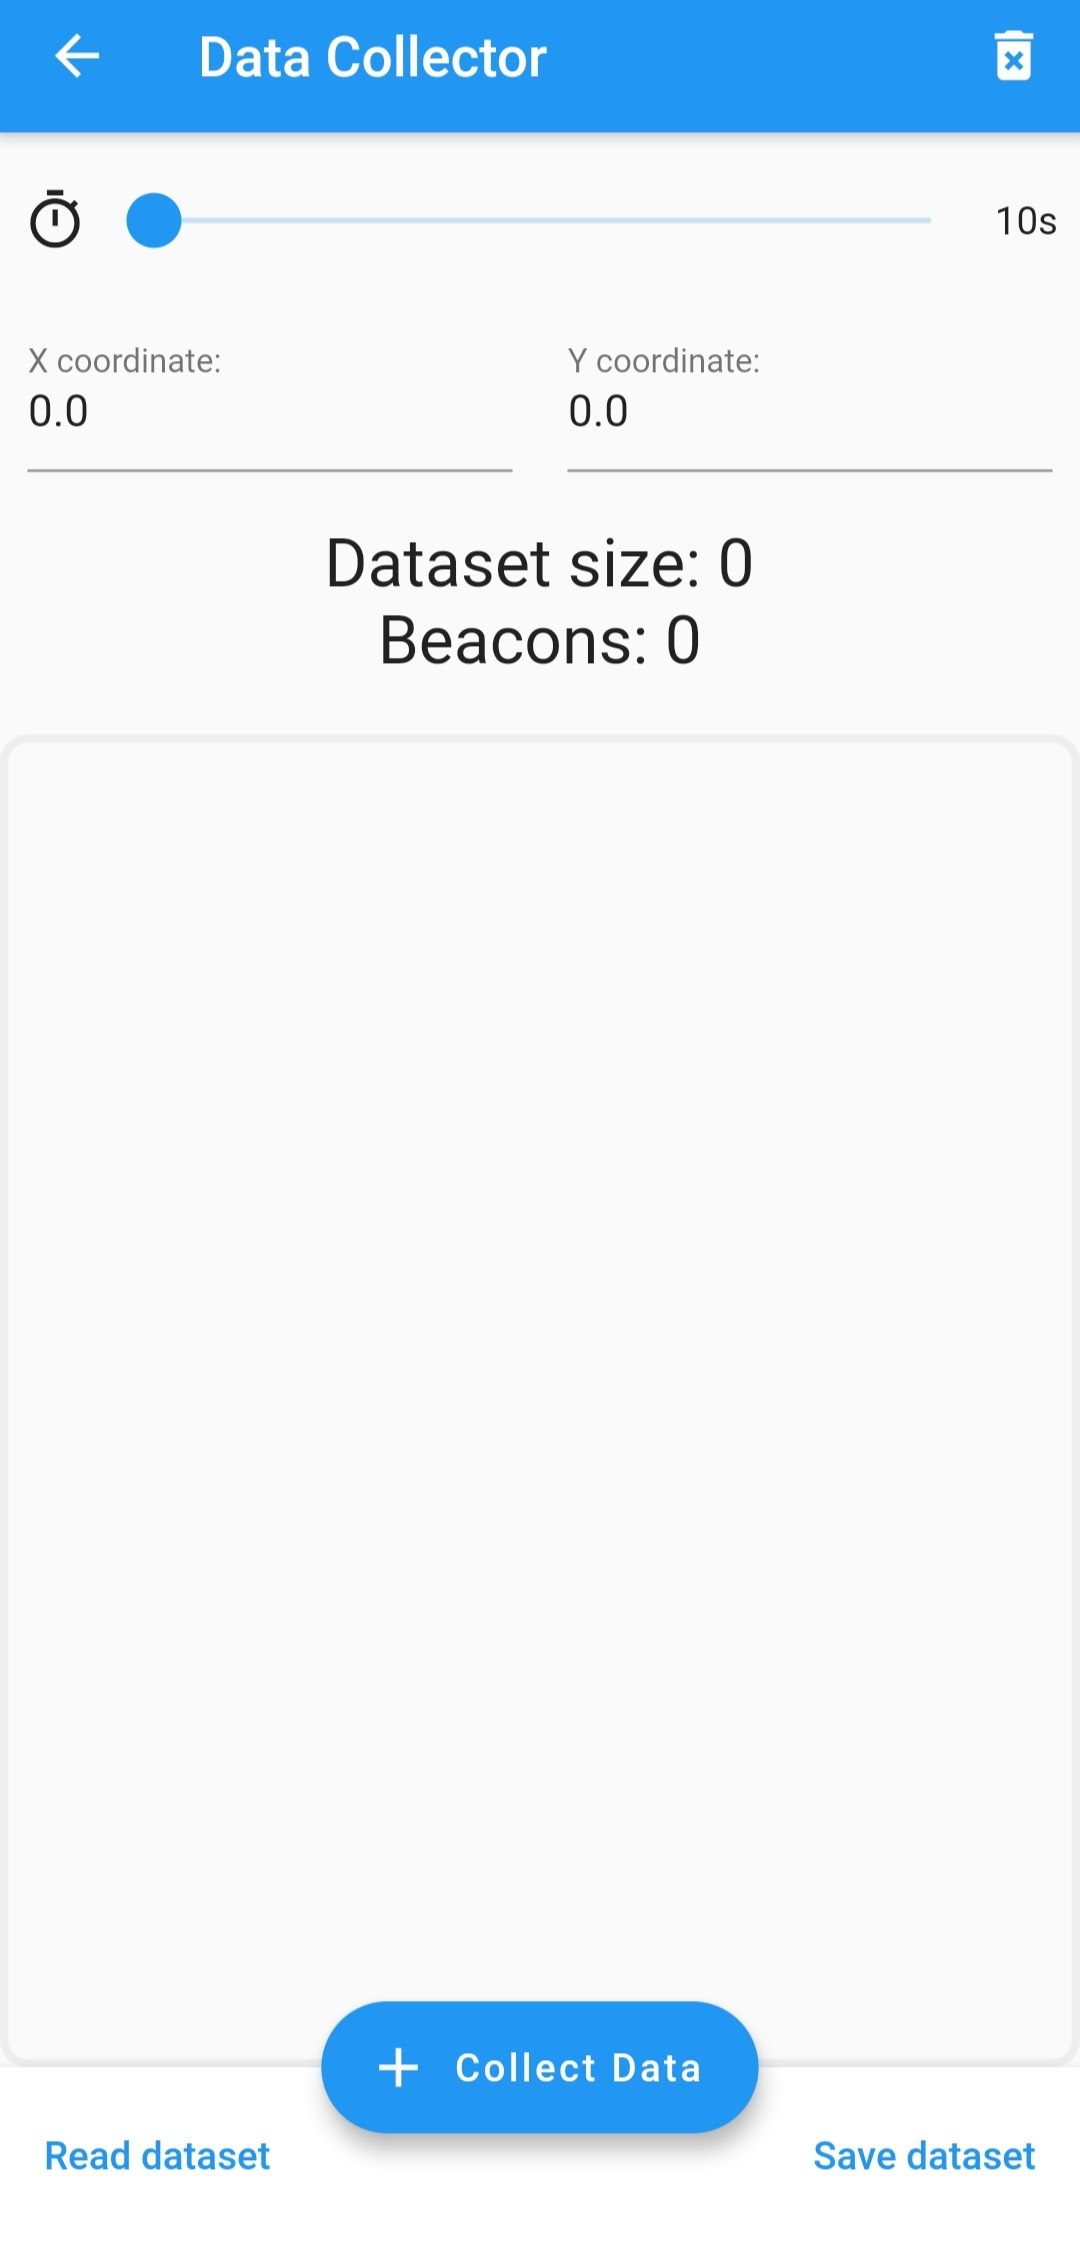
\includegraphics[width=\textwidth]{./img/screen-collector.jpg}%
      \caption{Raccolta dei segnali}
      \label{fig:collector}
    \end{subfigure}
    ~
    ~
    \begin{subfigure}{0.33\textwidth}
      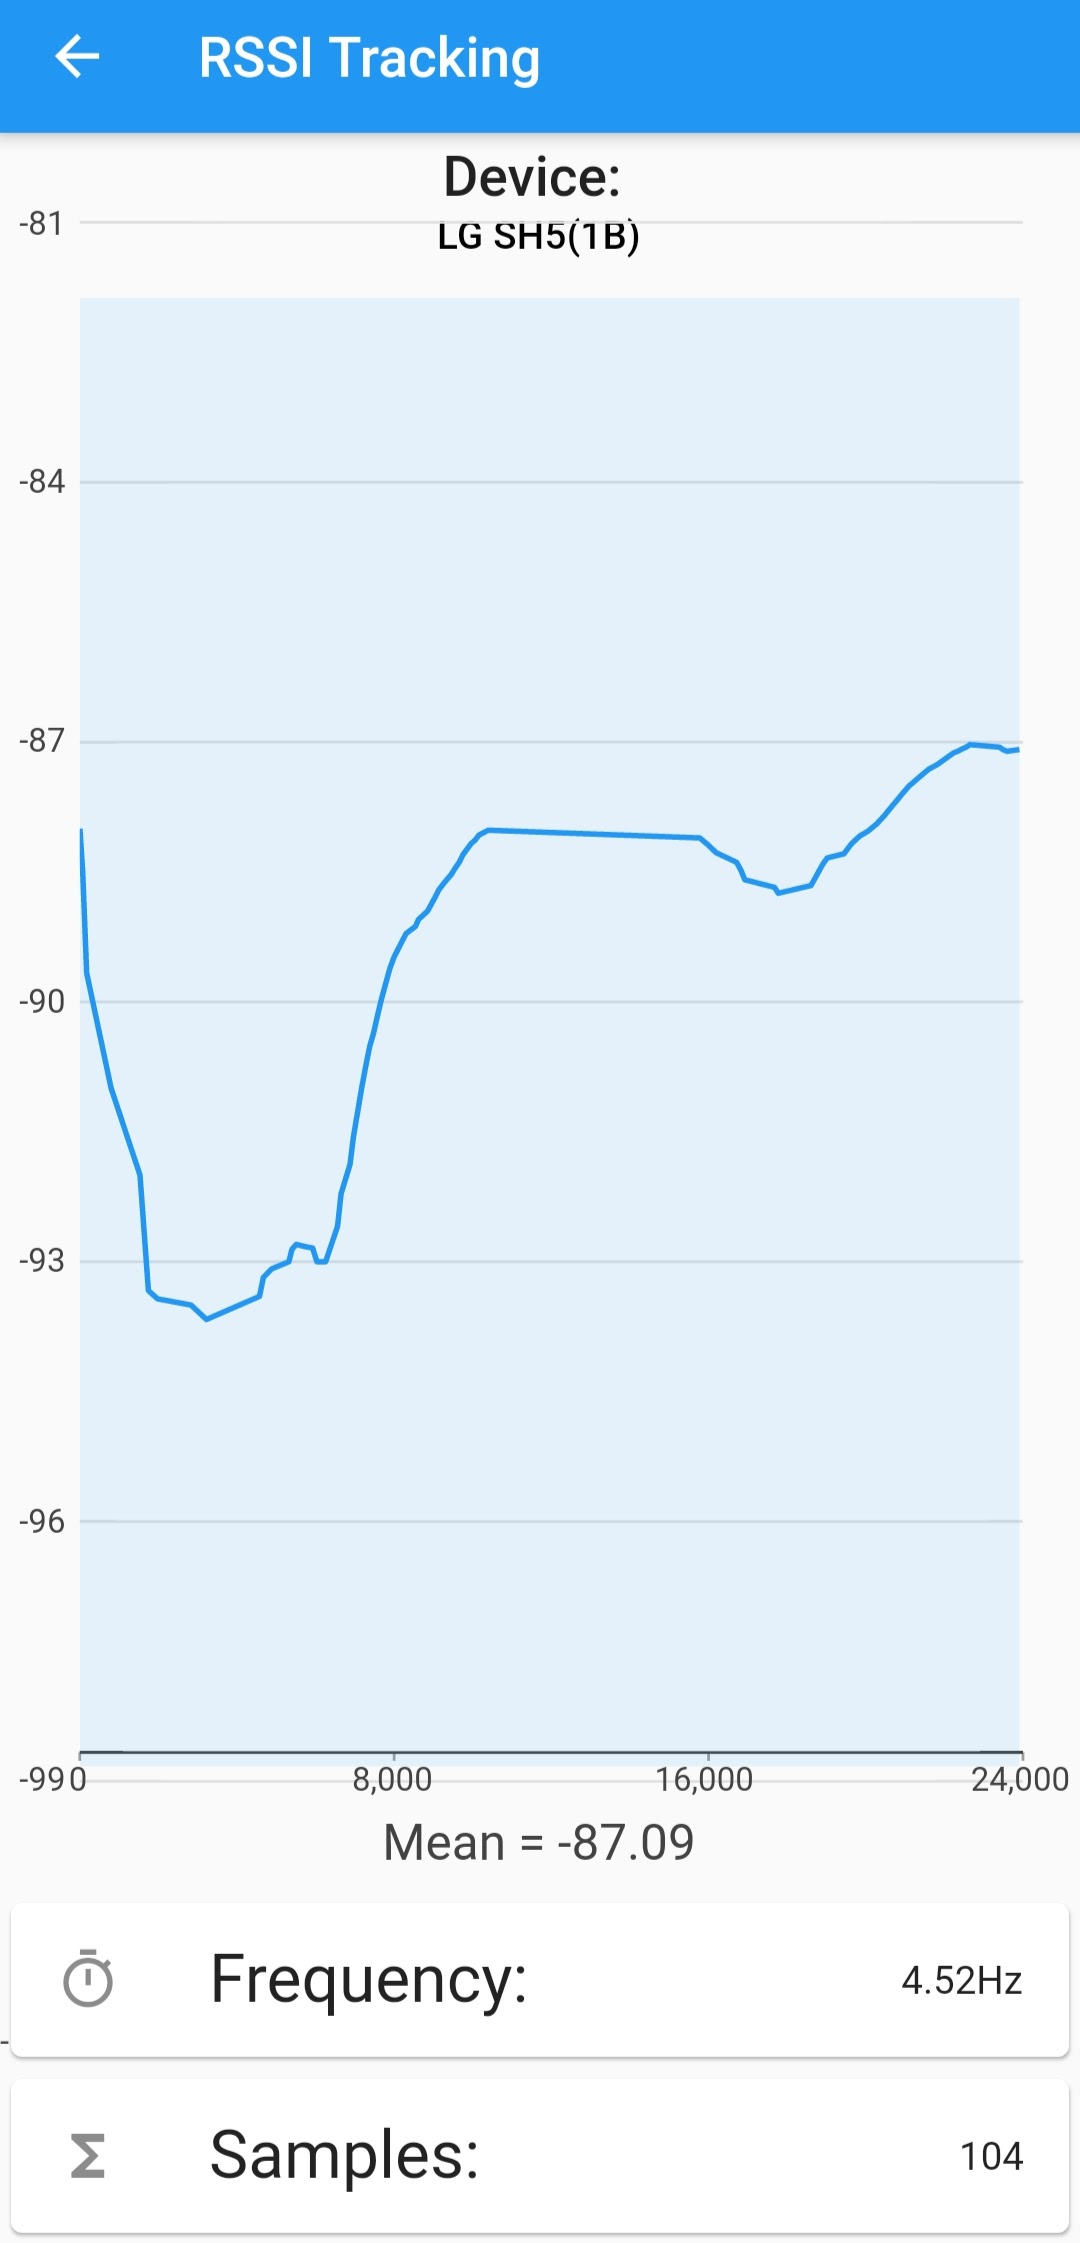
\includegraphics[width=\textwidth]{./img/screen-tracker.jpg}%
      \caption{Tracking dei segnali RSSI}
      \label{fig:tracker}
    \end{subfigure}
    ~
    ~
    \begin{subfigure}{0.33\textwidth}
      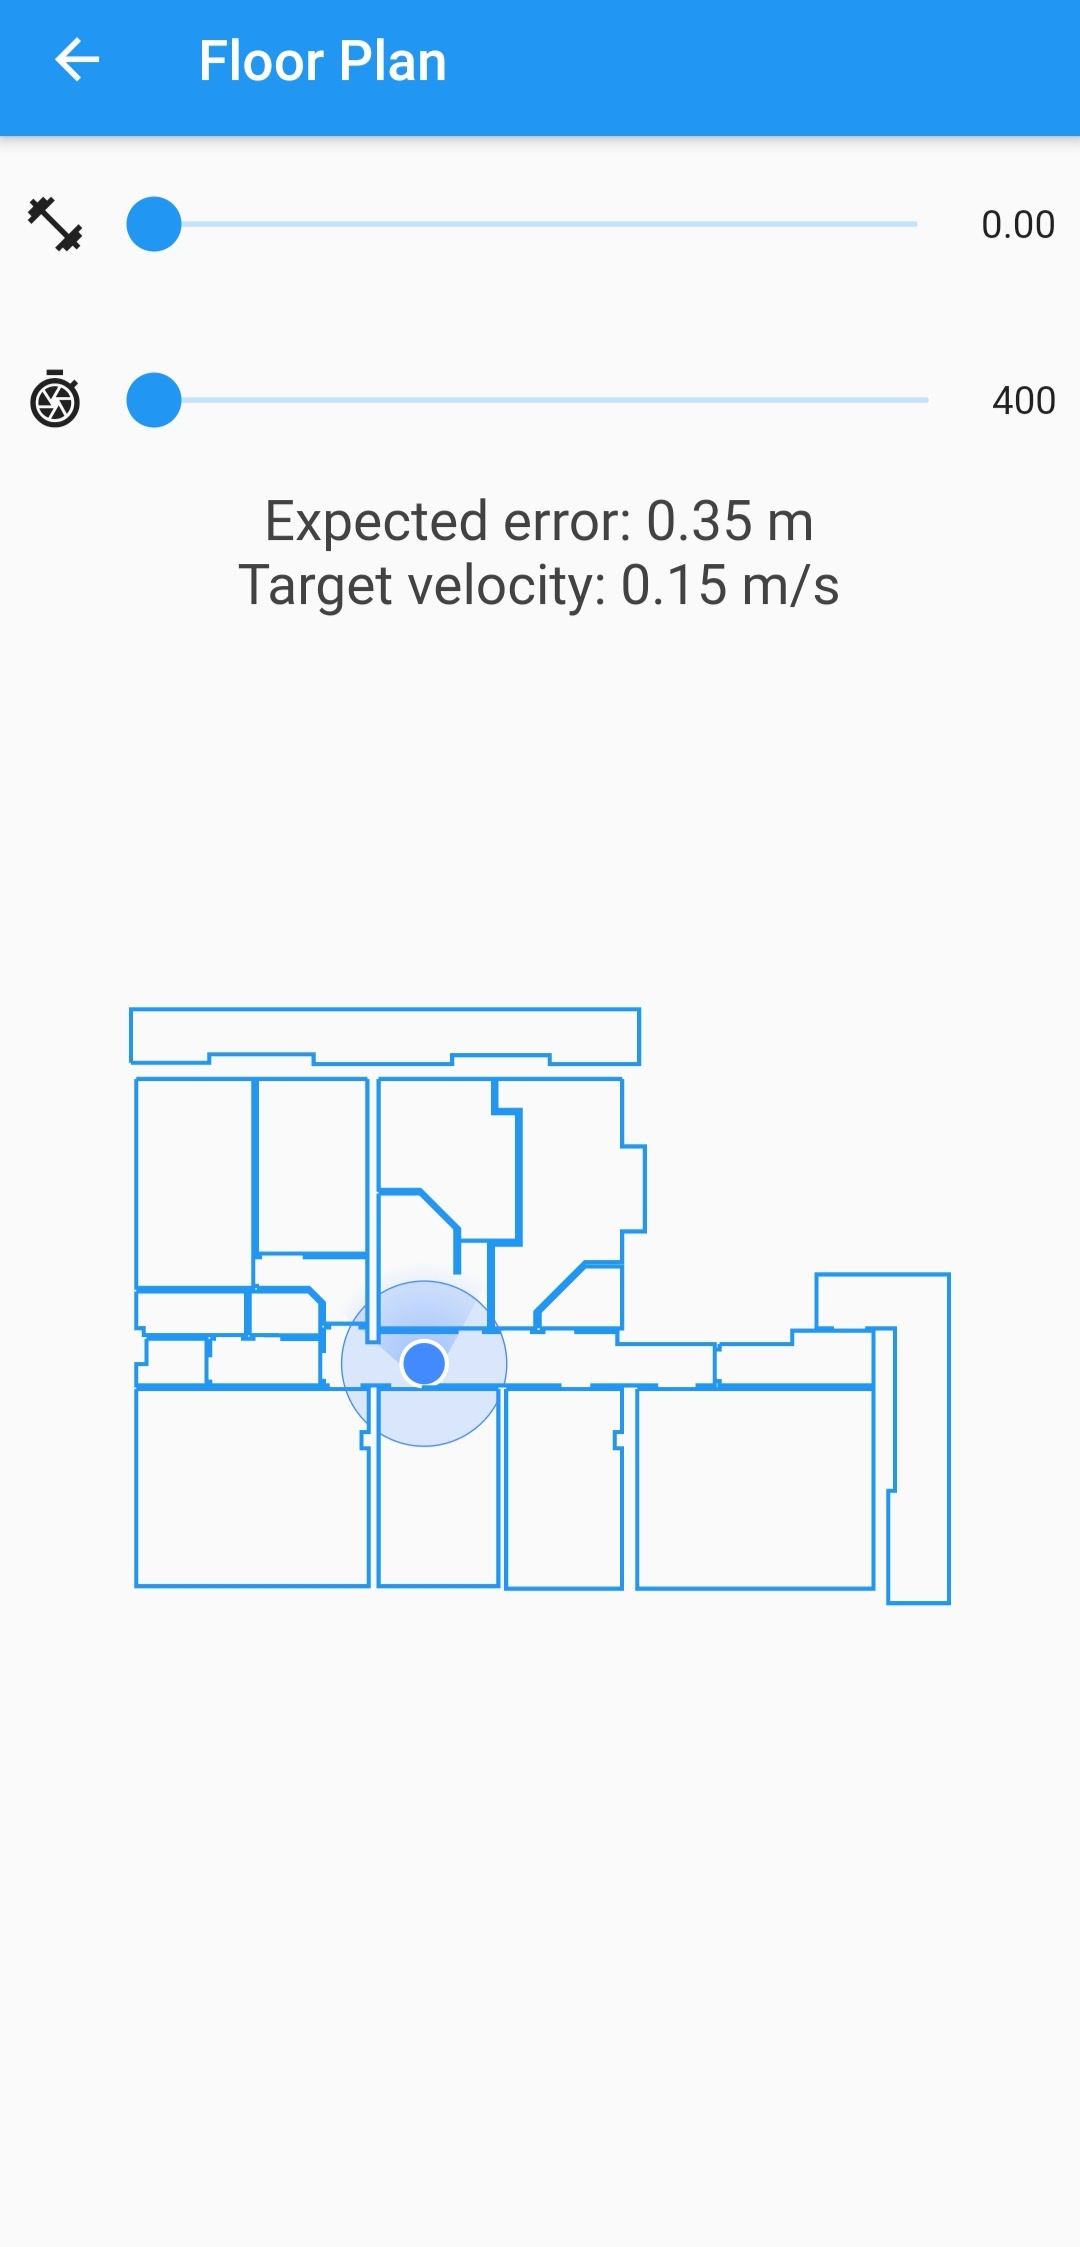
\includegraphics[width=\textwidth]{./img/screen-floorplan.jpg}%
      \caption{Visualizzatore Planimetrie}
      \label{fig:floorplan}
    \end{subfigure}
  }%
  \caption{Screenshot delle varie schede dell'applicazione mobile.}%
  \label{fig:gui}%
\end{figure}
In Figura~\ref{fig:collector} è mostrata la scheda relativa alla raccolta dei
dati. Essa permette di indicare le coordinate
del punto da cui si intende raccogliere i segnali Bluetooth e la lunghezza del
periodo di tempo del campionamento. L'interfaccia permette poi di salvare i
dati nella memoria interna del dispositivo in formato CSV, dopo essere stati
processati. La frequenza di campionamento è fissa e pari alla massima frequenza
disponibile per la ricerca di dispositivi Bluetooth in Android.

In Figura~\ref{fig:tracker} è illustrata la componente grafica
dell'applicazione sviluppata per lo studio dei segnali Bluetooth; Il suo
utilizzo è stato per lo più prototipale e inizialmente utile a valutare
l'andamento dei segnali emessi dai dispositivi Bluetooth in ambienti chiusi. Il
grafico mostra l'andamento in tempo reale della media dei valori RSSI raccolti
dall'applicazione per uno specifico dispositivo Bluetooth. In basso sono
indicati il numero di campionamento la frequenza con cui questi vengono
effettuati.

La Figura~\ref{fig:floorplan} mostra il visualizzatore di planimetrie: in alto
sono presenti due slider che gestiscono rispettivamente il coefficiente di
memoria residua del modello (Paragrafo \ref{subsec:input}) e la frequenza di
campionamento dei segnali.  Il visualizzatore è stato sviluppato senza
utilizzare asset predefiniti e la grafica del cursore è di tipo vettoriale.
\end{document}
